\section{Présentation de l’organisme d’accueil}
\subsection{Présentation de HPS}
Hightech Payment Systems (HPS) est une multinationale, leader dans l'édition des solutions de paiement électronique pour les institutions financières, processeurs, switches nationaux et régionaux dans le monde entier. Le groupe est aujourd’hui présent sur quatre continents, avec plus de 400 clients opèrent dans 90 pays en Europe, en Asie, au Moyen-Orient, en Afrique et aux Amériques.
\begin{figure}[h!]  
  \centering
    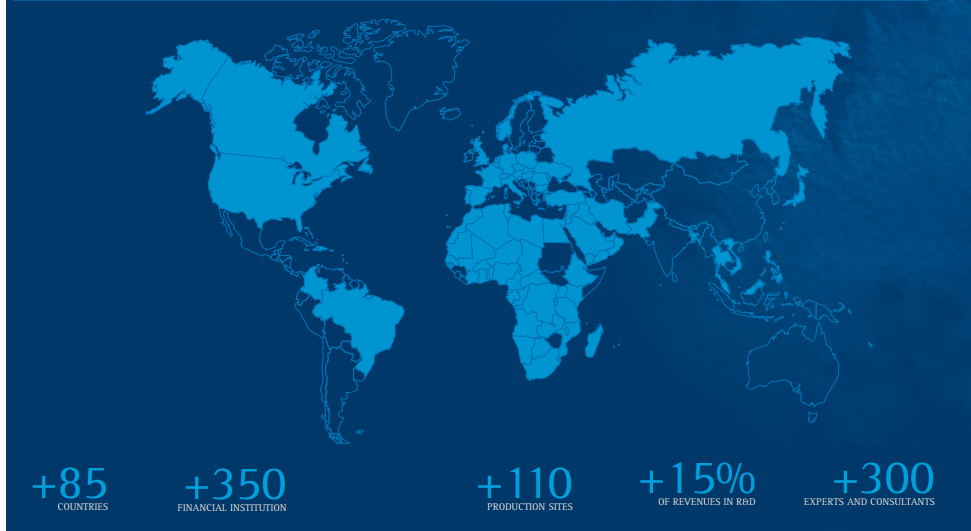
\includegraphics[width=0.8\textwidth]{chapitre1/Figures/presentationGeoHps.png}
  \caption{Présence Mondiale}
\end{figure}

\subsection{Fiche technique de l’entreprise}
%\begin{tabular}{|l|l|}
\begin{table}[!h]
\begin{tabular}{|p{4cm}||p{7cm}|}
\hline
Raison sociale & Hightech Payment Systems (HPS) \\
\hline
Siège social & Casablanca Nearshore Park, Shore 1 - Sector A, 1100 Bd Al Quods, Sidi Maârouf, Casablanca 20270, Maroc. \\
\hline
Forme juridique & Société Anonyme \\
\hline
Contact  & Tel : +212 529 045 000\\
& Fax : +212 529 014 096/97\\
& Mail : mail@hps-worldwide.com\\
& Site web: http://www.hps-worldwide.com\\
\hline
Date de création  & Janvier 1995 \\
\hline
Capital social  & 353 000 000 MAD \\
\hline
Effectif   & 385 \\
\hline
Secteur d’activité  & Monétique : fournisseur de solutions de paiement électronique multi-canal. \\
\hline
\end{tabular}
\centering \caption{Fiche technique de HPS} \label{TablePR}
\end{table}
\subsection{Organigramme HPS SOLUTIONS}
L’organisation d’HPS se découvre au travers cet organigramme. Celui-ci, conformément à ses objectifs stratégiques, s’organise en plusieurs pôles et directions métier.
\begin{figure}[h!]  
  \centering
    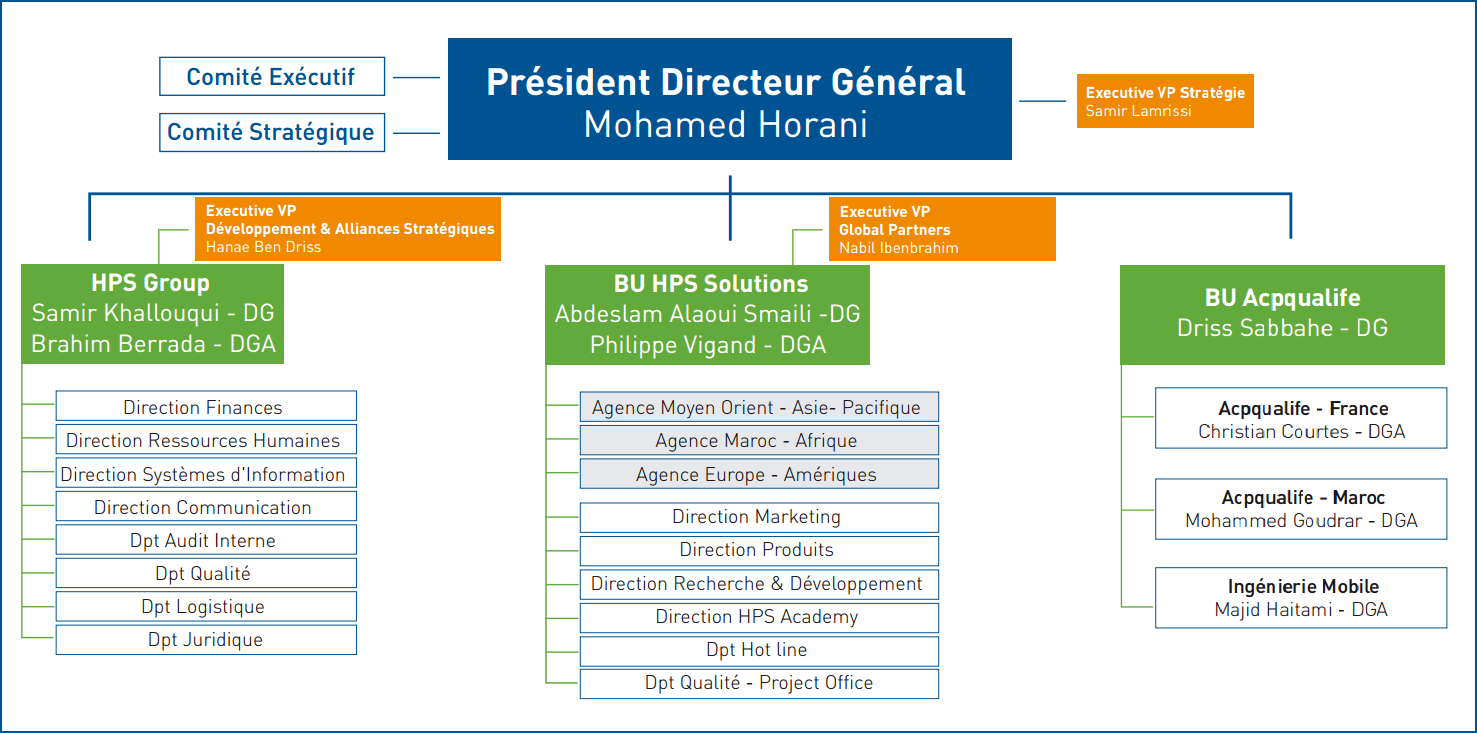
\includegraphics[width=1.1\textwidth]{chapitre1/Figures/organigrameHpsSolution.png}
  \caption{Organigramme HPS SOLUTIONS}
\end{figure}
\subsection{Présentation des secteurs d’activités}
Le progiciel Power CARD offert par HPS est une solution de paiement électronique évoluée et hautement sécurisée. Cette solution couvre l’intégralité de la chaîne de traitement les transactions financières liées au paiement électronique. Le produit est structuré en trois suites de solutions :\\
\ul{FrontOffice :}\\
Cette suite gère le pilotage des terminaux et guichets automatiques. Elle assure notamment les fonctions de sécurité et de vérification, la communication avec les moyens d’acquisition (TPE, GAB, Internet, etc.), la collecte et l’autorisation des transactions ainsi que la gestion des commerçants et des parcs de terminaux d’acquisition, etc.\\
\underline{Middle-Office :}\\
Cette deuxième suite assure le lien entre l’acquéreur et l’émetteur pour l’octroi d’autorisations, et le routage dans le cadre d’une interopérabilité nationale et/ou internationale, etc.\\
\underline{Back-Office :}\\
C’est la suite qui assure la gestion de l’émission de tout type de cartes (crédit, débit, prépayée, fidélité, etc.), la gestion de la personnalisation des cartes, la gestion de l’acquisition par les commerçants, la compensation (nationale et internationale), la gestion des litiges, le reporting, l’alimentation de la comptabilité des émetteurs et acquéreurs, etc.
\subsection{Présentation du service de stage}
On a passé notre stage au sein de l'agence Asie - Moyen orient, sous l'encadrement du Directeur de projet de l'agence qui a pour mission de piloter un ou plusieurs projets, de la phase de négociation préalable à la signature du contrat jusqu'à l'achèvement du projet en passant par le choix des ressources.
\newpage
\begin{figure}[h!]  
  \centering
    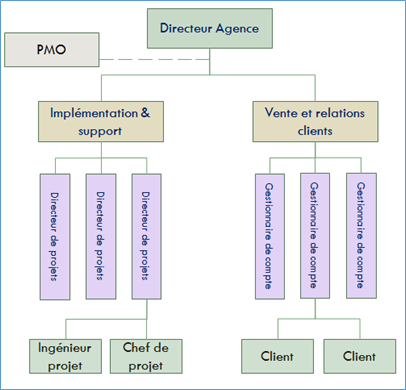
\includegraphics[width=0.7\textwidth]{chapitre1/Figures/AMAAF.png}
  \caption{Organigramme Agence Asie - Moyen orient}
\end{figure}
\subsection{Clients de l’agence Asie - Moyen orient}
\begin{figure}[h!]  
  \centering
    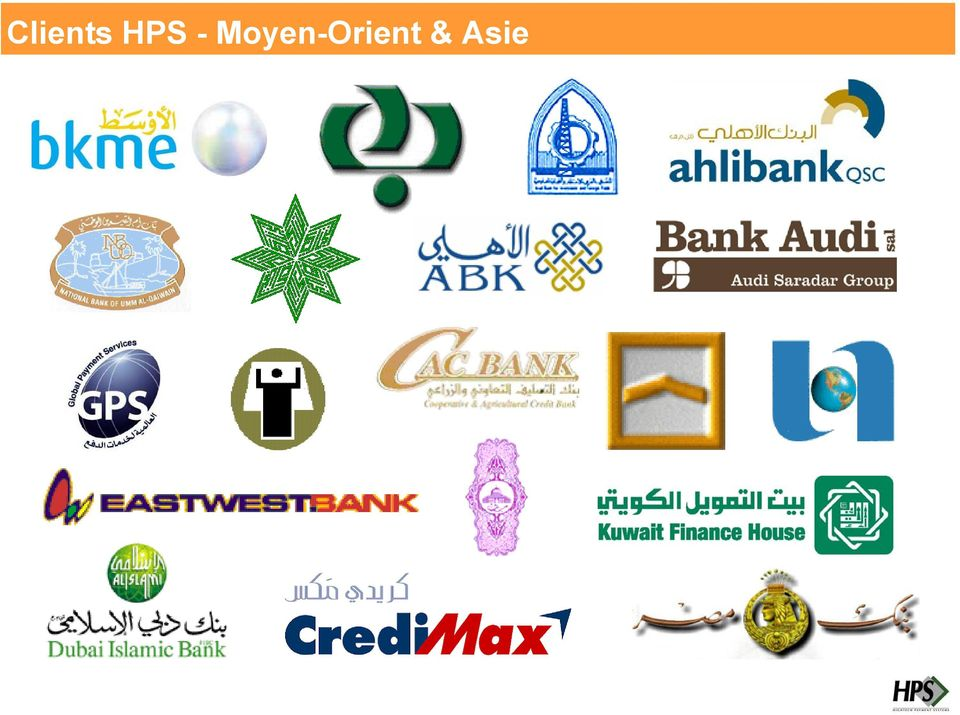
\includegraphics[width=0.7\textwidth]{chapitre1/Figures/clientMAAF.png}
  \caption{Clients de l’agence Asie - Moyen orient}
\end{figure}